% Provenance (never printed): cycle 4 SVT, "La planete Terre, l'environnement
% et l'action humaine": climate, its past variations and the present change,
% read from data; see sources/book1/PROVENANCE.md. Book 1, grade 9, chapter 1.
% Vocabulary guard: owns climate change (first look; Book 2 g12 re-uses it),
% global warming, temperature anomaly. The greenhouse effect and greenhouse
% gases belong to the chemistry series (grade 8): recalled in prose, never
% defined. Infrared is physics (g10): named in prose only. "Glacial period"
% and "interglacial" belong to Book 2 g12: here "the ice ages and the warmer
% times between them". Physical science only, in the IPCC's calibrated words;
% no policy.
\chapter{El clima de la Tierra, ayer y hoy}\label{ch:g9:climate-past-and-present}

Si la Tierra no tuviera aire a su alrededor, pero reflejara la misma
proporción de luz solar que hoy, su superficie se estabilizaría en una
temperatura media de unos \qty{-19}{\degreeCelsius}: \omterm{def:g2:water-on-earth:ocean}{mares} helados, tierras
heladas, por todas partes. Su media real es de unos
\qty{15}{\degreeCelsius}. La diferencia, unos \qty{34}{\degreeCelsius},
procede de unos pocos gases del aire, presentes en cantidades minúsculas,
que impiden que una parte del calor de la Tierra escape al espacio. Este
capítulo trata de esos gases, del \omterm{def:g5:weather-and-climate:climate}{clima} de la Tierra en el pasado y de
cómo y por qué está cambiando ahora.
% ledger: earth:Tbb, earth:Tsurf (figdata/grade-9/climate_records.py: -19.1 and 14.9 degC, gap 34)

\begin{recall}
El \omterm{def:g5:weather-and-climate:climate}{clima} de un lugar es el \omterm{def:g1:watching-the-weather:weather}{tiempo} que hace allí habitualmente, promediado
a lo largo de 30 años (\cref{ch:g5:weather-and-climate}). La capa más baja
de la atmósfera, donde ocurren los fenómenos meteorológicos, es la
\omterm{def:g8:the-atmosphere:layers}{troposfera} (\cref{ch:g8:the-atmosphere}). Las \omterm{def:g8:ice-on-earth:ice-age}{glaciaciones}, con \omterm{def:g8:ice-on-earth:ice-sheet}{inlandsis}
mucho más allá de los \omterm{def:g3:continents-and-oceans:poles}{polos}, han ido y venido; el \omterm{def:g8:ice-on-earth:sea-ice}{hielo marino} ártico ha
disminuido desde 1979 (\cref{ch:g8:ice-on-earth}). En química se aprende
que el dióxido de carbono, el metano y el vapor de agua son \emph{gases de
efecto invernadero}: dejan pasar la luz solar, pero absorben la luz
infrarroja invisible que emite el suelo caliente, y eso es el
\emph{efecto invernadero}; quemar carbón, petróleo y gas libera dióxido de
carbono.
\end{recall}

\section{El efecto invernadero y la temperatura de la Tierra}

La luz solar atraviesa la atmósfera y calienta el suelo y los \omterm{def:g2:water-on-earth:ocean}{océanos}.
Como todo cuerpo caliente, la superficie caliente emite a su vez energía,
en forma de luz infrarroja que el ojo no puede ver. Si toda ella escapara
al espacio, la Tierra sería el mundo helado del primer párrafo. Pero los
gases de efecto invernadero del aire absorben buena parte de esa luz
infrarroja y devuelven una parte hacia abajo: la superficie recibe energía
a la vez del Sol y del aire que tiene encima, y se estabiliza en una
temperatura más alta.

\begin{omfigure}
\begin{tikzpicture}[font=\footnotesize, >={Stealth[length=2.4mm]}]
  % ground and atmosphere
  \fill[omLithAlluv] (0,0) rectangle (12,0.5);
  \fill[omSea!45] (0,0.5) rectangle (12,3.4);
  \node[anchor=north east, align=right] at (11.85,3.35) {atmósfera con gases\\ de efecto invernadero};
  \node[anchor=south east] at (11.9,0.05) {suelo y océanos};
  \node[anchor=south west] at (0.15,3.5) {espacio};
  % Sun
  \fill[omWxSun] (1.3,5.0) circle (0.45);
  \node at (1.3,4.3) {Sol};
  % sunlight in
  \draw[->, omWxSun!80!black, line width=2.2pt] (1.7,4.6) -- (2.7,0.55)
    node[pos=0.25, right=2pt, align=left, black] {la luz solar entra\\ y calienta la superficie};
  % infrared out and back
  \draw[->, omWarm, line width=1.6pt, decorate, decoration={snake, amplitude=1mm, segment length=4mm, post length=3mm}]
    (6.0,0.55) -- (6.6,2.6);
  \draw[->, omWarm, line width=1.6pt, decorate, decoration={snake, amplitude=1mm, segment length=4mm, post length=3mm}]
    (6.6,2.7) -- (7.4,5.0) node[right, align=left, black] {una parte escapa\\ al espacio};
  \draw[->, omWarm, line width=1.6pt, decorate, decoration={snake, amplitude=1mm, segment length=4mm, post length=3mm}]
    (6.8,2.75) -- (8.6,0.55);
  \node[align=left, anchor=west] at (8.8,1.9) {una parte la absorben\\ los gases y la\\ devuelven hacia abajo};
  \node[align=right, anchor=east] at (5.9,1.3) {la superficie caliente\\ emite infrarrojo};
\end{tikzpicture}

{\small El efecto invernadero, de forma simplificada (un esquema). Sin él,
la superficie de la Tierra tendría una media de unos
\qty{-19}{\degreeCelsius}; con él, de unos \qty{15}{\degreeCelsius}.}
% ledger: earth:Tbb, earth:Tsurf
\label{fig:g9:climate-past-and-present:greenhouse}
\end{omfigure}

El efecto invernadero es natural y necesario: sin él no habría agua
líquida en la superficie. La pregunta de este capítulo es otra: ¿qué le
ocurre a la temperatura de la Tierra cuando cambia la cantidad de gases de
efecto invernadero del aire?

\section{Los climas del pasado}

Para leer el \omterm{def:g5:weather-and-climate:climate}{clima} de un pasado lejano, los científicos perforan los
\omterm{def:g8:ice-on-earth:ice-sheet}{inlandsis}. Cada año cae \omterm{def:g4:clouds-rain-snow:precipitation}{nieve} sobre la Antártida y Groenlandia, y la \omterm{def:g4:clouds-rain-snow:precipitation}{nieve}
de verano es un poco distinta de la de invierno. Enterradas y comprimidas
hasta convertirse en hielo, las capas anuales permanecen, una encima de
otra, como las páginas de un libro. Cuanto más profundo es el hielo, más
antiguo es.
% ledger: eo:ice-core

\begin{omfigure}
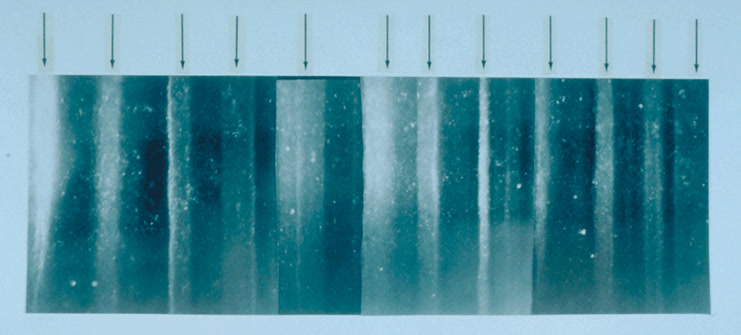
\includegraphics[width=0.78\linewidth]{images/book1/g9-gisp2-layers.jpg}

{\small Un tramo de testigo de hielo de \qty{19}{cm} de largo, extraído a
\qty{1855}{m} de profundidad en el \omterm{def:g8:ice-on-earth:ice-sheet}{inlandsis} de Groenlandia e iluminado
desde abajo. Las flechas señalan las capas de verano, más claras, entre
capas de invierno más oscuras: once años de \omterm{def:g4:clouds-rain-snow:precipitation}{nieve}. NOAA Paleoclimatology
(dominio público, vía Wikimedia Commons).}
% ledger: commons:gisp2-layers
\label{fig:g9:climate-past-and-present:ice-core}
\end{omfigure}

Un testigo de hielo guarda dos registros del pasado. La propia \omterm{def:g4:clouds-rain-snow:precipitation}{nieve}
indica lo frío que estaba el aire cuando cayó: cuanto más frío el aire,
menor es la proporción de las formas más pesadas del hidrógeno y del
oxígeno en la \omterm{def:g4:clouds-rain-snow:precipitation}{nieve}. Y a medida que la \omterm{def:g4:clouds-rain-snow:precipitation}{nieve} se comprime en hielo, los
espacios entre los granos se cierran y atrapan diminutas burbujas del
aire de la época. Los científicos liberan ese aire antiguo en el
laboratorio y miden su dióxido de carbono.
% ledger: eo:ice-core

\begin{omfigure}
\begin{tikzpicture}
\begin{axis}[name=temp, omrecord, omage, width=13cm, height=3.9cm, xmin=0, xmax=800,
  xtick={0,100,...,800}, xticklabels={}, ylabel={cambio de\\ temperatura ($^\circ$C)},
  ylabel style={align=center}, ymin=-11, ymax=5, ytick={-10,-5,0,5}]
  \addplot[omWarm, line width=0.7pt] table[x=age_kyr, y=temp_C] {figdata/out/grade-9-climate_records-edc.dat};
\end{axis}
\begin{axis}[at={(temp.south west)}, anchor=north west, yshift=-0.3cm, omrecord, omage,
  width=13cm, height=3.9cm, xmin=0, xmax=800, xtick={0,100,...,800},
  xlabel={miles de años antes de hoy}, ylabel={dióxido de carbono\\ (ppm)},
  ylabel style={align=center}, ymin=160, ymax=320, ytick={180,220,260,300}]
  \addplot[black, line width=0.7pt] table[x=age_kyr, y=co2_ppm] {figdata/out/grade-9-climate_records-icecore.dat};
\end{axis}
\end{tikzpicture}

{\small Ochocientos mil años leídos en el hielo de la Antártida. Arriba:
el cambio de la temperatura del aire en el Domo~C, respecto de la media de
los últimos mil años (testigo de hielo EPICA Domo~C, J.~Jouzel y otros,
2007). Abajo: el dióxido de carbono del aire atrapado en el hielo, en
partes por millón (B.~Bereiter y otros, 2015). Ambos promediados por
tramos de \num{2000} años; el tiempo avanza de izquierda (lo más antiguo) a
derecha (hoy).}
% ledger: data:edc-jouzel, data:co2-bereiter (figdata/grade-9/climate_records.py)
\label{fig:g9:climate-past-and-present:icecore}
\end{omfigure}

Las dos curvas cuentan la misma historia. Una y otra vez, largas épocas
frías, las \omterm{def:g8:ice-on-earth:ice-age}{glaciaciones}, dieron paso a épocas cálidas más cortas, y luego
volvió el frío. En los momentos más fríos, el aire sobre la Antártida
estaba unos \qty{9}{\degreeCelsius} más frío que en los últimos mil años;
en las épocas más cálidas, unos pocos grados más cálido. Y el dióxido de
carbono subía y bajaba con la temperatura, entre unos \qty{175}{ppm} en las
épocas frías y unos \qty{300}{ppm} en las cálidas. Vivimos en una de las
épocas cálidas, que empezó cuando terminó la última \omterm{def:g8:ice-on-earth:ice-age}{glaciación}.
% ledger: data:edc-jouzel, data:co2-bereiter (figdata/grade-9/climate_records.py: edc min -9.7, max +3.6; CO2 174 to 299 ppm)

\begin{method}[Leer dos registros uno junto al otro]
\begin{enumerate}
  \item Comprueba que los dos registros comparten el mismo eje del tiempo,
        y en qué sentido avanza el tiempo.
  \item Elige una fecha en el eje del tiempo y lee cada registro en esa
        fecha.
  \item Busca picos y \omterm{def:g1:landscapes-around-us:landform}{valles}: ¿aparecen en los mismos momentos en los dos
        registros?
  \item Di qué varía a la vez, sin decidir todavía qué cambio causó el
        otro.
\end{enumerate}
\end{method}

\begin{example}[La última glaciación en el testigo de hielo]
Hace \num{20000} años (el 20 del eje del tiempo), la curva de temperatura
está en unos \qty{-9}{\degreeCelsius} y el dióxido de carbono en unos
\qty{190}{ppm}. En los últimos mil años, la curva de temperatura está
cerca de 0 y el dióxido de carbono cerca de \qty{280}{ppm}. Así pues, en
el momento más frío de la última \omterm{def:g8:ice-on-earth:ice-age}{glaciación}, el aire sobre la Antártida
estaba unos \qty{9}{\degreeCelsius} más frío y contenía unos
$280 - 190 = \qty{90}{ppm}$ menos de dióxido de carbono, un tercio menos.
\end{example}
% ledger: data:edc-jouzel, data:co2-bereiter (figdata/grade-9/climate_records.py: 19-21 kyr bins -9.4, 190 ppm; 1 kyr bin 278)

Más atrás todavía, la Tierra conoció \omterm{def:g5:weather-and-climate:climate}{climas} mucho más cálidos que los de
cualquier momento de los últimos 800\,000 años. Las evaluaciones
científicas estiman que la última vez que la superficie de la Tierra se
mantuvo \qty{2.5}{\degreeCelsius} o más por encima de su nivel de finales
del siglo XIX fue hace más de tres millones de años.
% ledger: ipcc:3myr

\section{Los registros actuales}

Desde finales del siglo XIX, la temperatura se mide cada día en miles de
\omterm{def:g4:clouds-rain-snow:weather-station}{estaciones meteorológicas} en tierra y en el \omterm{def:g2:water-on-earth:ocean}{mar}, con termómetros
resguardados a la sombra. Para seguir el planeta entero, los científicos
no promedian las propias temperaturas, que dependen de dónde está cada
estación, sino cuánto se aparta cada una de su propio valor habitual.
% ledger: giss:method

\begin{definition}[Anomalía de temperatura]\label{def:g9:climate-past-and-present:anomaly}
Una \emph{anomalía de temperatura}\index{anomalia de temperatura@anomalía de temperatura} es la diferencia
entre una temperatura y su media a lo largo de un periodo de referencia
elegido. Es positiva cuando hace más calor que esa media y negativa cuando
hace más frío.
\end{definition}

\begin{omfigure}
\begin{minipage}[c]{0.44\linewidth}\centering
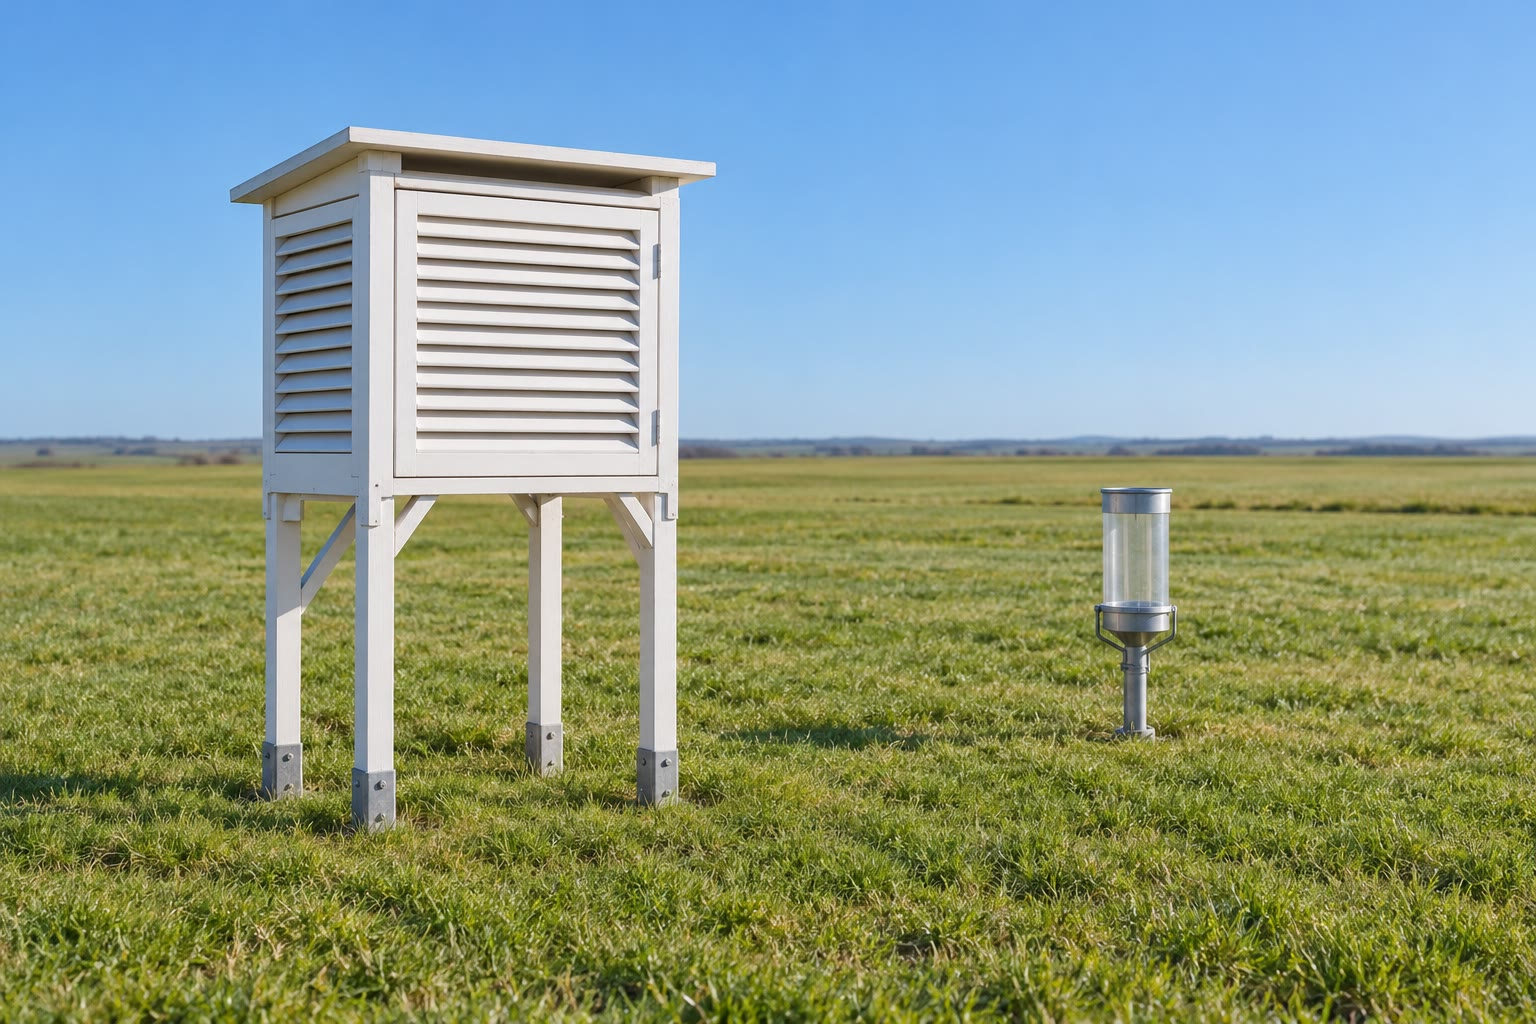
\includegraphics[width=\linewidth]{images/book1/ai/g9-weather-screen.jpg}
\end{minipage}\hfill
\begin{minipage}[c]{0.52\linewidth}\raggedright
{\small Una \omterm{def:g4:clouds-rain-snow:weather-station}{estación meteorológica}: la caseta blanca sobre patas, de
paredes de lamas, mantiene los termómetros a la sombra mientras el aire
circula a través de ella; a la derecha, un \omterm{def:g4:clouds-rain-snow:rain-gauge}{pluviómetro} (ilustración
generada por IA de una escena genérica).}
\end{minipage}
\label{fig:g9:climate-past-and-present:screen}
\end{omfigure}

El registro de la temperatura global de la NASA, por ejemplo, da la
anomalía de cada año respecto de la media de 1951--1980, a partir de
estaciones en tierra y de medidas de la superficie del \omterm{def:g2:water-on-earth:ocean}{mar}. Promediado
década a década, muestra una clara subida.
% ledger: giss:method, data:gistemp

\begin{omfigure}
\begin{tikzpicture}
\begin{axis}[omrecord, ybar, width=13cm, height=5.6cm, bar width=9pt,
  ymin=-0.45, ymax=1.2, ytick={-0.4,0,0.4,0.8,1.2},
  xtick=data, xticklabels={1880--89, 1890--99, 1900--09, 1910--19, 1920--29, 1930--39, 1940--49, 1950--59, 1960--69, 1970--79, 1980--89, 1990--99, 2000--09, 2010--19, 2020--25},
  x tick label style={rotate=60, anchor=east, font=\scriptsize},
  ylabel={anomalía de temperatura ($^\circ$C)}, xmajorgrids=false]
  \addplot[fill=omWarm!70, draw=black!50] table[x expr=\coordindex, y=mean_C]
    {figdata/out/grade-9-climate_records-decades.dat};
\end{axis}
\end{tikzpicture}

{\small La temperatura de la superficie del planeta, década a década desde
la de 1880, en forma de anomalía respecto de la media de 1951--1980; la
última barra abarca los seis años 2020--2025. Datos: NASA GISTEMP,
versión~4.}
% ledger: data:gistemp (figdata/grade-9/climate_records.py)
\label{fig:g9:climate-past-and-present:decades}
\end{omfigure}

\begin{definition}[Calentamiento global]\label{def:g9:climate-past-and-present:global-warming}
El \emph{calentamiento global}\index{calentamiento global} es la subida de
la temperatura media de la superficie de la Tierra, en su conjunto, desde
la segunda mitad del siglo XIX.
\end{definition}

Año a año, el registro sube y baja: un año puede ser más frío que el
anterior, porque el \omterm{def:g1:watching-the-weather:weather}{tiempo} de todo un año, sobre \omterm{def:g2:water-on-earth:ocean}{océanos} y \omterm{def:g3:continents-and-oceans:continent}{continentes},
también varía. Para medir un calentamiento, los científicos comparan, por
tanto, medias de muchos años, nunca dos años sueltos.

\begin{omfigure}
\begin{tikzpicture}
\begin{axis}[omrecord, width=13cm, height=5.4cm, xmin=1875, xmax=2030, ymin=-0.6, ymax=1.4,
  xtick={1880,1900,...,2020}, x tick label style={/pgf/number format/1000 sep={}},
  xlabel={año}, ylabel={anomalía de temperatura ($^\circ$C)},
  legend style={at={(0.2,0.97)}, anchor=north west, draw=none, fill=white, font=\footnotesize}]
  \fill[omWarm!10] (axis cs:1880,-0.6) rectangle (axis cs:1899,1.4);
  \fill[omWarm!10] (axis cs:2015,-0.6) rectangle (axis cs:2024,1.4);
  \addplot[black!70, mark=*, mark size=0.9pt, line width=0.4pt]
    table[x=year, y=anomaly_C] {figdata/out/grade-9-climate_records-annual.dat};
  \addlegendentry{cada año}
  \addplot[omWarm, line width=2pt] table[x=year, y=mean_C] {figdata/out/grade-9-climate_records-periods.dat};
  \addlegendentry{media de un periodo}
  \draw[dashed, black!50] (axis cs:1875,0) -- (axis cs:2030,0);
  \node[font=\scriptsize, fill=white, inner sep=1pt] at (axis cs:1889.5,0.45) {1880--1899};
  \node[font=\scriptsize, fill=white, inner sep=1pt] at (axis cs:2019.5,0.3) {2015--2024};
\end{axis}
\end{tikzpicture}

{\small La anomalía de la temperatura global de cada año de 1880 a 2025
(respecto de la media de 1951--1980, línea discontinua), con las medias de
dos periodos del problema de este capítulo: 1880--1899 y 2015--2024.
Datos: NASA GISTEMP, versión~4.}
% ledger: data:gistemp (figdata/grade-9/climate_records.py)
\label{fig:g9:climate-past-and-present:annual}
\end{omfigure}

\begin{method}[Medir un calentamiento entre dos periodos]
\begin{enumerate}
  \item Elige dos periodos de al menos diez años cada uno, uno al
        principio y otro al final, para que los altibajos de los años
        sueltos se compensen.
  \item Calcula la media de las anomalías anuales de cada periodo.
  \item Resta la media del primero de la del segundo: el resultado es el
        calentamiento entre los dos periodos, en grados.
  \item Di qué registro y qué periodos has usado: otro registro, u otros
        periodos, dan un número algo distinto.
\end{enumerate}
\end{method}

\begin{example}[El calentamiento desde la década de 1970]
En el registro de la NASA, las anomalías de los diez años 1970--1979
tienen una media de \qty{0.03}{\degreeCelsius}, y las de 2010--2019, de
\qty{0.80}{\degreeCelsius}. El calentamiento entre esas dos décadas es de
$0.80 - 0.03 = \qty{0.77}{\degreeCelsius}$, en cuarenta años: unos
\qty{0.19}{\degreeCelsius} por década. Dos años sueltos, también separados
por cuarenta años, darían respuestas muy distintas: 1976 ($-0.10$) frente a
2016 (1.01) da \qty{1.11}{\degreeCelsius}, pero 1979 (0.16) frente a 2011
(0.61) solo da \qty{0.45}{\degreeCelsius}.
\end{example}
% ledger: data:gistemp (figdata/grade-9/climate_records.py: decade_1970s 0.03, decade_2010s 0.80; annual 1976 -0.10, 2016 1.01, 1979 0.16, 2011 0.61)

El dióxido de carbono del aire se mide directamente desde marzo de 1958,
en un observatorio situado a unos \qty{3400}{m} de \omterm{def:g4:world-physical-map:altitude}{altitud} en las laderas
del \omterm{def:g4:volcanoes-earthquakes-first-look:volcano}{volcán} Mauna Loa, en Hawái. En 1959, su media anual era de
\qty{316}{ppm}; en 2025 había llegado a \qty{427}{ppm}, muy por encima de
los \qty{300}{ppm} que nunca superó en 800\,000 años de hielo. Sube cada
vez más deprisa: menos de \qty{1}{ppm} al año en la década de 1960, más de
\qty{2.5}{ppm} al año en los últimos diez años.
% ledger: gml:keeling, data:co2-mlo, data:co2-bereiter (figdata/grade-9/climate_records.py: 315.98, 427.35, 0.86 and 2.63 ppm/yr; ice core max 298.6)

\begin{omfigure}
\begin{tikzpicture}
\begin{axis}[omrecord, width=12cm, height=5cm, xmin=1955, xmax=2030,
  ymin=290, ymax=440, ytick={300,350,400}, xtick={1960,1970,...,2020},
  x tick label style={/pgf/number format/1000 sep={}},
  xlabel={año}, ylabel={dióxido de carbono (ppm)}]
  \addplot[black, line width=0.9pt, mark=*, mark size=0.8pt] table[x=year, y=co2_ppm] {figdata/out/grade-9-climate_records-co2.dat};
  \draw[dashed, omWarm] (axis cs:1955,300) -- (axis cs:2030,300);
\end{axis}
\end{tikzpicture}

{\small El dióxido de carbono del aire en Mauna Loa, Hawái, medias anuales
1959--2025 (NOAA Global Monitoring Laboratory y Scripps Institution of
Oceanography). La línea discontinua de \qty{300}{ppm} corresponde
aproximadamente al nivel más alto hallado en 800\,000 años de hielo
antártico.}
% ledger: data:co2-mlo, data:co2-bereiter (figdata/grade-9/climate_records.py)
\label{fig:g9:climate-past-and-present:co2}
\end{omfigure}

\begin{dated}{2025}
La media anual del dióxido de carbono en Mauna Loa fue de
\qty{427.35}{ppm} en 2025. En el registro de la NASA, el año más cálido
desde 1880 fue 2024, con una anomalía de \qty{1.28}{\degreeCelsius}
respecto de 1951--1980.
% ledger: data:co2-mlo, data:gistemp (figdata/grade-9/climate_records.py)
\end{dated}

El \omterm{def:g2:water-on-earth:ocean}{mar} también sube. Desde 1993, los satélites miden la altura de la
superficie del \omterm{def:g2:water-on-earth:ocean}{mar} en todo el \omterm{def:g3:continents-and-oceans:globe}{globo}: la línea de tendencia de su registro
sube unos \qty{3.2}{mm} al año, unos \qty{10}{cm} en treinta años. Dos
cosas hacen subir el \omterm{def:g2:water-on-earth:ocean}{mar}: el agua que se calienta se dilata, y el hielo
continental que se funde añade agua al \omterm{def:g2:water-on-earth:ocean}{océano}. Y el hielo está
disminuyendo: los \omterm{def:g8:ice-on-earth:glacier}{glaciares} de \omterm{def:g1:landscapes-around-us:landform}{montaña} retroceden casi en todas partes, y
el \omterm{def:g8:ice-on-earth:sea-ice}{hielo marino} de verano del Ártico ha perdido casi la mitad de su
extensión desde 1979 (\cref{ch:g8:ice-on-earth}).
% ledger: data:gmsl-lsa (figdata/grade-9/climate_records.py: 3.18 mm/yr; 101 mm 1993-2024), ipcc:b1-ice, nsidc:ice-shelves, data:b1-nsidc-sea-ice

\begin{omfigure}
\begin{tikzpicture}
\begin{axis}[omrecord, width=12cm, height=4.8cm, xmin=1992, xmax=2026,
  ymin=-30, ymax=100, xtick={1995,2000,...,2025},
  x tick label style={/pgf/number format/1000 sep={}},
  xlabel={año}, ylabel={nivel del mar (mm)},
  legend style={at={(0.02,0.97)}, anchor=north west, draw=none, fill=white, font=\footnotesize}]
  \addplot[omCold, mark=*, mark size=1.1pt, line width=0.6pt] table[x=year, y=gmsl_mm] {figdata/out/grade-9-climate_records-sea.dat};
  \addlegendentry{media anual}
  \addplot[omWarm, dashed, line width=0.9pt] table[x=year, y=gmsl_mm] {figdata/out/grade-9-climate_records-sea-trend.dat};
  \addlegendentry{línea de tendencia}
\end{axis}
\end{tikzpicture}

{\small El nivel medio global del \omterm{def:g2:water-on-earth:ocean}{mar} medido por satélite, medias anuales
1993--2024, respecto de un nivel de referencia, y su línea de tendencia
(NOAA Laboratory for Satellite Altimetry).}
% ledger: data:gmsl-lsa (figdata/grade-9/climate_records.py)
\label{fig:g9:climate-past-and-present:sea}
\end{omfigure}

\section{El cambio climático y sus causas}

\begin{definition}[Cambio climático]\label{def:g9:climate-past-and-present:climate-change}
El \emph{cambio climático}\index{cambio climatico@cambio climático} es un
cambio del \omterm{def:g5:weather-and-climate:climate}{clima} de la Tierra, o de una región, que dura décadas o más: un
cambio de su temperatura media, de sus \omterm{def:g4:clouds-rain-snow:precipitation}{lluvias}, de sus vientos o de su
hielo, y no una sola estación fuera de lo común.
\end{definition}

El \omterm{def:g5:weather-and-climate:climate}{clima} siempre ha cambiado, como muestran los testigos de hielo. Lo
nuevo es la rapidez del cambio actual, y su causa. Científicos de todo el
mundo evalúan periódicamente lo que se ha publicado sobre el \omterm{def:g5:weather-and-climate:climate}{clima} en los
informes del Grupo Intergubernamental de Expertos sobre el Cambio
Climático (IPCC). Los informes sopesan el grado de certeza de cada
afirmación, con palabras escogidas con cuidado.

En estos informes, cada una de las expresiones siguientes tiene un
significado fijo: las posibilidades sobre 100 de que la afirmación sea
cierta.

\begin{center}
{\small
\begin{tabular}{|l|c||l|c|}
\hline
\emph{prácticamente seguro} & 99 a 100 & \emph{probable} & 66 a 100 \\
\emph{sumamente probable} & 95 a 100 & \emph{tan probable como improbable} & 33 a 66 \\
\emph{muy probable} & 90 a 100 & \emph{improbable} & 0 a 33 \\
\hline
\end{tabular}}
\end{center}
% ledger: ipcc:likelihood

\noindent Unas pocas afirmaciones no llevan ninguna de estas expresiones:
se dan como hechos, como ``es \emph{inequívoco}''. Cuando leas una noticia
sobre el \omterm{def:g5:weather-and-climate:climate}{clima}, busca estas expresiones y fíjate en cuáles conserva la
noticia y cuáles omite.
% ledger: ipcc:unequivocal

La evaluación publicada en 2021 afirma lo siguiente.
\begin{itemize}
  \item Es \emph{inequívoco} que la influencia humana ha calentado la
        atmósfera, el \omterm{def:g2:water-on-earth:ocean}{océano} y la tierra.
  \item La temperatura de la superficie del planeta en 2011--2020 fue
        unos \qty{1.1}{\degreeCelsius} más alta que en 1850--1900, y cada
        una de las cuatro últimas décadas fue más cálida que cualquier
        década anterior desde 1850.
  \item El calentamiento causado por el ser humano entre 1850--1900 y
        2010--2019 está \emph{probablemente} entre 0.8 y
        \qty{1.3}{\degreeCelsius}, con una estimación central de
        \qty{1.07}{\degreeCelsius}: aproximadamente todo el calentamiento
        observado. Las causas naturales en conjunto modificaron la
        temperatura solo entre $-0.1$ y $+\qty{0.1}{\degreeCelsius}$.
  \item El dióxido de carbono del aire en 2019 era más alto que en
        cualquier momento de al menos los dos últimos millones de años
        (\emph{confianza alta}); había aumentado un 47~\% desde 1750.
  \item Es \emph{muy probable} que la influencia humana sea la causa
        principal del retroceso de los \omterm{def:g8:ice-on-earth:glacier}{glaciares} desde la década de 1990 y
        de la disminución del \omterm{def:g8:ice-on-earth:sea-ice}{hielo marino} ártico; y \emph{muy probable}
        que sea la causa principal de la subida del \omterm{def:g2:water-on-earth:ocean}{mar} desde al menos
        1971.
\end{itemize}
% ledger: ipcc:unequivocal, ipcc:gsat-2011-2020, ipcc:decades, ipcc:attribution, ipcc:co2-2myr, ipcc:b1-ice, ipcc:sea-level-obs

\begin{history}[La curva de Charles David Keeling]
En marzo de 1958, un joven químico de la Scripps Institution of
Oceanography, Charles David Keeling, empezó a medir el dióxido de carbono
del aire en el Mauna Loa, muy por encima del \omterm{def:g2:water-on-earth:ocean}{mar} y lejos de cualquier
ciudad. Sus medidas han continuado desde entonces: son el registro más
largo de dióxido de carbono medido directamente en el aire, y la curva que
dibujan, que sube año tras año, lleva su nombre: la \emph{curva de
Keeling}.
% ledger: gml:keeling
\end{history}

¿Por qué sigue el calentamiento al dióxido de carbono? Quemar carbón,
petróleo y gas libera dióxido de carbono; más dióxido de carbono en el aire
significa que se absorbe y se devuelve hacia abajo una parte mayor de la
luz infrarroja que emite la superficie, y la superficie se calienta. El
vapor de agua, el metano y los demás gases de efecto invernadero se suman
al efecto. El pasado y el presente coinciden: en los testigos de hielo
como en los registros actuales, la temperatura de la Tierra y su dióxido
de carbono suben y bajan a la vez.
% ledger: ipcc:attribution, ipcc:co2-2myr

\section{Ejercicios}

\begin{exercise}[$\star$]\label{exo:g9:climate-past-and-present:1}
% ledger: earth:Tbb, earth:Tsurf
(a) ¿Cuál sería la temperatura media de la superficie de la Tierra sin el
efecto invernadero? (b) ¿Cuál es con él? (c) ¿Cuántos grados calienta la
superficie el efecto invernadero? (d) Nombra dos gases de efecto
invernadero.
\end{exercise}

\begin{exercise}[$\star$]\label{exo:g9:climate-past-and-present:2}
¿\omterm{def:g1:watching-the-weather:weather}{Tiempo} o \omterm{def:g5:weather-and-climate:climate}{clima}? (a) Ayer llovió todo el día. (b) Los veranos de esta
región son calurosos y secos. (c) La década de 2010 fue más cálida que la
de 1980 en todo el mundo. (d) La semana que viene hará frío.
\end{exercise}

\begin{exercise}[$\star$]\label{exo:g9:climate-past-and-present:3}
% ledger: commons:gisp2-layers
Observa la fotografía del tramo de testigo de hielo. (a) ¿Cuánto mide el
tramo, y cuántos años de \omterm{def:g4:clouds-rain-snow:precipitation}{nieve} contiene? (b) Halla el espesor medio de la
capa de un año, en centímetros. (c) ¿Por qué el hielo más profundo de un
\omterm{def:g8:ice-on-earth:ice-sheet}{inlandsis} es el más antiguo?
\end{exercise}

\begin{exercise}[$\star$]\label{exo:g9:climate-past-and-present:4}
La temperatura media de julio de una ciudad en 1991--2020 es de
\qty{21.0}{\degreeCelsius}. Da la \omterm{def:g9:climate-past-and-present:anomaly}{anomalía de temperatura} de un mes de
julio con una media de (a) \qty{22.4}{\degreeCelsius};
(b) \qty{20.3}{\degreeCelsius}; (c) \qty{21.0}{\degreeCelsius}. (d) ¿Qué
significa una anomalía negativa?
\end{exercise}

\begin{exercise}[$\star\star$]\label{exo:g9:climate-past-and-present:5}
% ledger: data:gistemp (figdata/grade-9/climate_records.py)
Usa el diagrama de barras de las décadas. (a) ¿Qué décadas fueron más frías
que la media de 1951--1980? (b) Lee la anomalía de la década de 1980 y la
de la década de 2010. (c) ¿Cuánto creció la anomalía entre esas dos
décadas? (d) ¿Es regular la subida de una década a la siguiente a lo largo
de todo el registro?
\end{exercise}

\begin{exercise}[$\star\star$]\label{exo:g9:climate-past-and-present:6}
% ledger: data:co2-mlo (figdata/grade-9/climate_records.py)
En Mauna Loa, la media anual del dióxido de carbono fue de
\qty{315.98}{ppm} en 1959, \qty{324.62}{ppm} en 1969, \qty{401.01}{ppm} en
2015 y \qty{427.35}{ppm} en 2025. (a) ¿Cuál fue la subida media por año de
1959 a 1969? (b) ¿Y de 2015 a 2025? (c) ¿Cuántas veces más rápida fue la
subida en el segundo periodo? (d) ¿En qué porcentaje aumentó el dióxido de
carbono de 1959 a 2025?
\end{exercise}

\begin{exercise}[$\star\star$]\label{exo:g9:climate-past-and-present:7}
% ledger: data:edc-jouzel, data:co2-bereiter
Usa el registro de 800\,000 años. (a) Escribe 800\,000 años en notación
científica. (b) ¿Hace cuánto tiempo, aproximadamente, hizo tanto calor
como hoy por última vez, antes de nuestra propia época cálida? (c) ¿Qué
nivel de dióxido de carbono contenía el aire en aquella época? (d) ¿Suben
y bajan la temperatura y el dióxido de carbono en los mismos momentos?
\end{exercise}

\begin{exercise}[$\star\star$]\label{exo:g9:climate-past-and-present:8}
% ledger: data:gmsl-lsa (figdata/grade-9/climate_records.py)
El \omterm{def:g2:water-on-earth:ocean}{mar} sube unos \qty{3.2}{mm} al año. (a) ¿Cuánto es eso en 10 años, en
centímetros? (b) Si mantuviera este ritmo, ¿cuánto subiría entre 2025 y
2100? (c) Nombra dos razones por las que sube el \omterm{def:g2:water-on-earth:ocean}{mar}. (d) ¿Hace subir el
\omterm{def:g2:water-on-earth:ocean}{mar} la fusión del \omterm{def:g8:ice-on-earth:sea-ice}{hielo marino} ártico? Explícalo.
\end{exercise}

\begin{exercise}[$\star\star$]\label{exo:g9:climate-past-and-present:9}
% ledger: ipcc:likelihood
En las expresiones del IPCC, ¿cuántas posibilidades sobre 100, como
mínimo, tiene cada afirmación de ser cierta? (a) ``Es \emph{muy
probable}\ldots'' (b) ``Es \emph{probable}\ldots'' (c) ``Es
\emph{prácticamente seguro}\ldots'' (d) Un periódico escribe ``los
científicos están seguros de que'' sobre una afirmación que el informe
califica de \emph{probable}. ¿Qué falla?
\end{exercise}

\begin{exercise}[$\star\star$]\label{exo:g9:climate-past-and-present:10}
Un amigo dice: ``Este invierno ha sido el más frío de los últimos diez
años donde vivo, así que la Tierra no se está calentando''. Explica, usando
las palabras \emph{\omterm{def:g1:watching-the-weather:weather}{tiempo}}, \emph{\omterm{def:g5:weather-and-climate:climate}{clima}} y \emph{global}, por qué este
argumento no se sostiene.
\end{exercise}

\begin{exercise}[$\star\star\star$]\label{exo:g9:climate-past-and-present:11}
% ledger: data:co2-bereiter, data:co2-mlo, ipcc:co2-2myr, ipcc:erf-2xco2
En el momento más frío de la última \omterm{def:g8:ice-on-earth:ice-age}{glaciación}, hace unos
$2 \times 10^4$ años, el aire contenía unos \qty{190}{ppm} de dióxido de
carbono; justo antes de la era industrial, unos \qty{280}{ppm}; en 2025,
unos \qty{427}{ppm}. (a) ¿Cuánto subió el dióxido de carbono desde la
\omterm{def:g8:ice-on-earth:ice-age}{glaciación} hasta la era industrial, y en cuántos años? (b) ¿Cuánto subió
desde la era industrial hasta 2025? Toma 1750 como inicio de la era
industrial. (c) Compara las dos subidas: en magnitud y en ritmo medio por
año, usando la notación científica. (d) ¿Qué dice el IPCC sobre el nivel
actual de dióxido de carbono comparado con el del pasado?
\end{exercise}

\begin{exercise}[$\star\star\star$]\label{exo:g9:climate-past-and-present:12}
% ledger: ipcc:attribution, ipcc:observed-2010-2019
La evaluación del IPCC da para el calentamiento observado entre 1850--1900
y 2010--2019 un valor de unos \qty{1.06}{\degreeCelsius}, y para el
calentamiento causado por el ser humano, \emph{probablemente} entre 0.8 y
\qty{1.3}{\degreeCelsius} (estimación central \qty{1.07}{\degreeCelsius});
para las causas naturales en conjunto da entre
$-0.1$ y $+\qty{0.1}{\degreeCelsius}$. (a) Compara la estimación central
del calentamiento causado por el ser humano con el calentamiento
observado. (b) ¿Podrían las causas naturales explicar por sí solas el
calentamiento observado? Explícalo. (c) ¿Qué significa \emph{probablemente}
en esta frase?
\end{exercise}

\section{Problema: el termómetro del planeta}

\begin{problem}[{Problema de fin de semana --- se calcula el calentamiento
de la Tierra a partir del registro de temperatura de la NASA y se compara
después con el dióxido de carbono y con el mar}]
\label{pb:g9:climate-past-and-present:1}
% ledger: data:gistemp, data:co2-mlo, data:gmsl-lsa, ipcc:gsat-2011-2020 (figdata/grade-9/climate_records.py)
La tabla da la anomalía de la temperatura global del registro de la NASA
(respecto de la media de 1951--1980) para algunos grupos de años, junto
con otros registros del capítulo.

\begin{center}
{\small
\begin{tabular}{|l|c|}
\hline
anomalía media, 1880--1899 & \qty{-0.22}{\degreeCelsius} \\
anomalía media, 1951--1980 & \qty{0.00}{\degreeCelsius} \\
anomalía media, 2015--2024 & \qty{0.98}{\degreeCelsius} \\
dióxido de carbono en Mauna Loa, 1959 / 2025 & \qty{316}{ppm} / \qty{427}{ppm} \\
tendencia del \omterm{def:g4:world-physical-map:altitude}{nivel del mar} por satélite, desde 1993 & \qty{3.2}{mm} al año \\
\hline
\end{tabular}}
\end{center}

\noindent\textbf{Parte I --- Las décadas.}\par\nopagebreak
\begin{enumerate}[beginpenalty=10000]
  \item ¿Por qué la anomalía de 1951--1980 es exactamente cero?
  \item ¿Fue 1880--1899 más cálido o más frío que 1951--1980? ¿En cuánto?
  \item ¿Fue 2015--2024 más cálido o más frío que 1951--1980? ¿En cuánto?
  \item Calcula el calentamiento de 2015--2024 respecto de 1880--1899.
\end{enumerate}

\noindent\textbf{Parte II --- El dióxido de carbono.}\par\nopagebreak
\begin{enumerate}[resume, beginpenalty=10000]
  \item ¿Cuántas ppm subió el dióxido de carbono entre 1959 y 2025?
  \item ¿Qué porcentaje de su valor de 1959 representa esa subida?
  \item En los testigos de hielo, el dióxido de carbono nunca superó unos
        \qty{300}{ppm} en 800\,000 años. ¿En cuánto lo supera el valor de
        2025?
  \item Explica en dos frases cómo más dióxido de carbono en el aire
        calienta la superficie.
\end{enumerate}

\noindent\textbf{Parte III --- El mar.}\par\nopagebreak
\begin{enumerate}[resume, beginpenalty=10000]
  \item ¿Cuánto ha subido el \omterm{def:g2:water-on-earth:ocean}{mar} de 1993 a 2025 al ritmo de la tabla, en
        centímetros?
  \item Nombra las dos causas de esa subida.
  \item El IPCC da para el calentamiento de 2011--2020 respecto de
        1850--1900 un valor de unos \qty{1.09}{\degreeCelsius}. ¿Es tu
        respuesta a la pregunta~4 del mismo orden? Da una razón por la que
        los dos números difieren un poco.
  \item Escribe la frase que podría publicar un periodista científico:
        ``Desde finales del siglo XIX, la superficie de la Tierra se ha
        calentado unos \ldots''
\end{enumerate}
\end{problem}
